\chapter{Effect of dissipation versus reflection on drift force}
\label{appendix:reflectionversusdrift}

Consider a two-dimensional irrotational wave train in deep water, with amplitude $a$. According to mass transport velocity, the waves have an average horizontal momentum $I$, which for low waves is simply proportional to the square of the wave amplitude:
\begin{equation}
    I = \frac{1}{2} \rho g a^2/c
\end{equation}
Where $\rho$ is the water density, $g$ is the gravitational constant and $c$ is the phase velocity. Since in deep water the group velocity $c_g$ = $\frac{1}{2}c$, a horizontal momentum flux is expected as
\begin{equation}
    I c_g = \frac{1}{4}\rho g a^2
\end{equation}
per unit distance across the waves. 
\begin{figure}
    \centering
    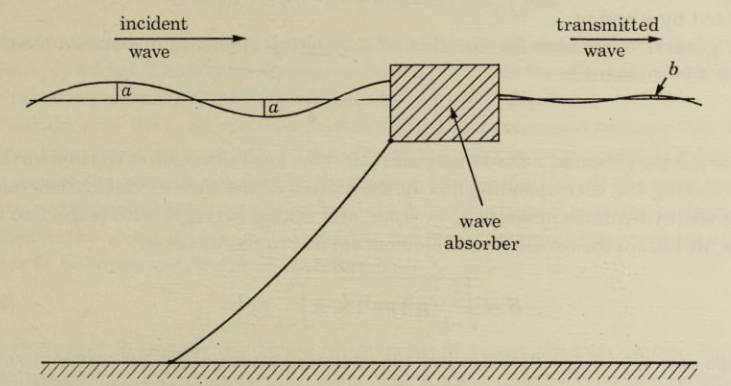
\includegraphics[width=0.7\linewidth]{figures/Literature_Introduction/waveabsorber_longuethiggins1977.PNG}
    \caption{Schematic representation of a wave absorber in a train of waves \parencite{longuethiggins1977}}
    \label{fig: wavetrainabsorber_longuetHiggins1977}
\end{figure}

Suppose this wave train is interacting with a floating body as schematically displayed in the figure\ref{fig: wavetrainabsorber_longuetHiggins1977}. Momentum is coming in with regard to the body, some momentum flux will be reflected and some of the momentum flux is transmitted through. In general, the body is expected to be subject to a force \parencite{longuethiggins1977}
\begin{equation}
    F = (Ic_g)_{in} + (Ic_g)_{ref} - (Ic_g)_{trans}
\end{equation}
per unit distance across the waves. In deep water this becomes
\begin{equation}
    F = \frac{1}{4} \rho g (a_i^2 + a_r^2 - a_t^2) 
    \label{eq: expected forizontal force on body}
\end{equation}
per unit distance across the waves. Here $a_i$ is the incident wave amplitude, $a_r$ is the reflected wave amplitude and $a_t$ is the transmitted wave amplitude. When no energy is absorbed by the floating body $(a_i^2=a_r^2 + a_t^2)$, this can be rewritten to
\begin{equation}
    F = \frac{1}{2} \rho g a_r^2 = \frac{1}{2} \rho g a_i^2(1-K_t^2)
\end{equation}
per unit distance across the waves. Here $K_t=a_t/a_i$ is the transmission coefficient. 
If the floating body would reflect the complete wave ($a_i=a_r, a_t=0$), the resulting horizontal force would be 

\begin{equation}
    F = \frac{1}{2} \rho g a_i^2
\end{equation}


per unit distance across the waves. If the floating body would adsorb all the wave energy ($a_r=0)$ then it must absorb the momentum also.  Hence we expect that it will be subject to a mean horizontal force of
\begin{equation}
    F = \frac{1}{4} \rho g a_i^2
\end{equation}
per unit distance across the waves. So, this absorbing floating body is experiencing a less horizontal force with factor two. \parencite{suyehiro1924drift} was the first who wrote about the existence of drift forces on ships caused by rolling among waves and also he attributed these forces to the reflection of the incoming waves by the model. \\
\\
In other words, attenuating the waves by reflection does not have a contribution to the lowering of the drift forces. Accordingly, the focus of designing the floating breakwaters for this application will be attenuating the waves by friction and dissipation as much as possible. \\
\\
On the other hand, the fender forces induced by the motion of the floating island is also a huge challenge. It does not matter for the reduction of motions of the structure whether the waves are attenuated through reflection, dissipation or friction. So reflecting the waves can be useful for the reduction of the motions of the floating island connected to the lee-side of the floating breakwater.
\\